% Celé zařízení je rozděleno na základní jednotku a~případné moduly, které zajistí nové herní možnosti.
% Například může jít o~připojení úložného prostoru nebo zvukového modulu, který poskytne jak plnohodnotný zvukový výstup tak vstup.

% \subsection{uživatelské požadavky}
Uživatelským požadavkem je statické zařízení sloužící jako herní stanoviště.
Vyžaduje tedy mobilitu jen v~rámci transportu na místo hry a~zpět, nikoliv v~rámci samotné hry.
Z~toho plynou požadavky na velikost výsledného zařízení.

Zařízení bude mít dva světelné kruhy složené z~60 inteligentních RGB LED.
Číslo 60 jsem zvolil, protože se jedná o~dostatečně jemné dělení, aby se daly dělat plynulé efekty.
Zároveň jde o~číslo, které koresponduje s~hodinovým ciferníkem a stupnicí na kompasu.
Jeden z~kruhů bude radiální a~druhý axiální.
Axiální je na horní straně zařízení a~slouží primárně jako odezva pro hráče na malou vzdálenost, např. při zadávání hesla.
Radiální kruh je pak také v~horní části zařízení a~slouží naopak pro signalizaci na delší vzdálenost, takový maják.

%TODO: dopsat a vygenerovat ilustraci
Uvnitř axiálního světelného kruhu se bude nacházet tzv. tlaková plocha.
\label{popisTlakovky} Jedná se o~ovládací prvek podobný dotykové ploše, s~tím rozdílem, že je schopen měřit i~sílu, která na něj působí.
Tento prvek je založen na měření rezonanční frekvence snímacích LC článků, nad kterými se nachází tlaková plocha.
Tlaková plocha je vodivý objekt, ve kterem se cívkou LC článku indukují vířivé proudy a následně se jimi indukují proudy zpět v cívce LC článku.
Tím plocha ovlivňuje indukčnost cívky a tedy i rezonanční frekvenci LC článku.
Ovlivnění indukčnosti je závislé na vzdálenosti plochy od cívky a tedy i na síle, která na plochu působí.
Velikost síly, která na plochu působí, totiž ovlivňuje její průhyb a tedy i vzdálenost od cívky.
Díky velkému rozlišení použitého čipu LDC1614 \cite{LDC1614} (28 bitů) je možné měřit změny vzdálenosti v řádu jednotek mikrometrů \cite{LDC1614LinearPositionSensing}.
Tato metoda je tedy schopna měřit vzdálenost plochy od jednotlivých cívek, které jsou čtyři, a plochu tak snímají na čtyřech místech.
Následně je z těchto hodnot možno dopočítat, jak je plocha nakloněna a tím určit, kde se jí uživatel dotýká.
% Protože je zároveň možné určit i sílu jakou uživatel při dotyku vyvinul, dostal tento systém jméno tlaková plocha. % silová by bývalo přesnější ale nějak mi to nejde přes pysky

Aby bylo stanoviště reálně použitelné při hře, musí celou hru vydržet na baterii.
Není ojedinělé, aby měla outdoorová hra čtyři až pět hodin bez přestávky.
Plus je nutná časová rezerva a~čas na nastavování.
Čas, který zařízení zvládne běžet z~baterie, silně závisí na činnosti, ale nebylo by zrovna ideální, kdyby byla baterka, výrazně omezujícím faktorem.
Výdrž na jedno nabití by tedy měla být alespoň pět hodin.

Vzhledem k~plánu připojovat moduly je nutné navrhnout mechanizmus připojení.
Bylo by ideální, kdyby si mohl uživatel říct co bude hrát za hru a~podle toho si sám připojil moduly, které potřebuje.
Tomuto určitě nechci bránit, ale přímo to podporovat nese řadu problémů, jak ze strany konektoru a~mechaniky, tak ze strany softwaru.
Konektor by totiž musel být ideálně beznástrojově rozpojitelný a~opětovně spojitelný a~přitom dostatečně pevný, aby se zařízení mechanicky chovalo jako jeden celek.
Takový konektor je ale poměrně složité udělat, tak aby byl spolehlivý, a~tak jde v~tuto chvíli jen o možnost dalšího vývoje.
Ze softwarového pohledu jde pak o~problém jak detekovat konkrétní modul a~hlavně o~otázku jak se chovat k~modulům, které jsou potenciálně záměnné.
Dejme tomu, že máme modul klávesnici a~modul dvířka.
Dvířka jsou původně navržena primárně jako úložný prostor, díky detekci zavření je lze ale použít i~jako velmi pohodlná tlačítka a~v~některých hrách se proto používají jen jako tlačítka.
Potenciální modul klávesnice je ovšem jen suma tlačítek.
Při vytváření konkrétní hry na míru modulům, které herní návrhář má zrovna k~dispozici, je tento problém nepodstatný, protože sám návrhář rozhodne, co má jak být.
Ale ve chvíli, kdy jde o~hru navrženou pro jinou kombinaci modulů, nastává problém jak rozhodnout, zda se dají dvířka použít místo klávesnice nebo ne.
Abych se všem těmto problémům alespoň prozatím vyhnul, rozhodl jsme se, že doplnění či výměna modulu, půjde jen při servisním zásahu.
Problém záměny modulů pak budu řešit tím, že každá hra bude vytvořena jen pro konkrétní sadu modulů.

Některé hry vyžadují tak velké herní území, že by na komunikaci mezi stanovištěmi už nestačila WiFi ani Bluetooth, které AHS jinak využívá ke komunikaci (viz: \ref{sec:TypVzdaleneKomunikace}).
Proto bude mít AHS možnost připojení k~mobilní síti a~tedy připojení k~internetu (výběr viz: \ref{sec:TypVzdaleneKomunikace}).
Tím se rozšíří dosah AHS všude, kde je mobilní pokrytí a~také přibude další metoda jak se stanovištěm komunikovat.
V~rámci tohoto komunikačního modulu bude možné používat navíc i~GNSS \footnote{Global Navigation Satellite System}.
Vzhledem k~faktu, že se přece jen nejedná o~systém, který by využila většina her a~zároveň je poměrně drahý, došel jsem k~rozhodnutí mít jej jen jako doplnitelný modul.
Protože se ale jedná o~modul, který zprostředkovává komunikaci se světem, je pravděpodobné, že bude potřebovat převádět výrazně větší množství dat než běžný modul.
Primárně z~tohoto důvodu je tento modul připojen na samostatném konektoru, přímo uvnitř základního zařízení.
Potřebné antény mohou být už v~základním zařízení, ale samotný modul spadá do doplňkové výbavy.

V~řadě případů je užitečné mít možnost zvukové zpětné vazby.
Ideální by bylo moci přehrávat libovolnou nahrávku, většinou ale stačí jednoduchý tón, řekněme jako potvrzení zadaného hesla.
Možnost přehrávat plnohodnotnou nahrávku proto odsouvám na samostatný modul a~v základní jednotce pro jednoduchost postačí piezoměnič nebo podobná sirénka.

Z~požadavků mi vyplynulo zařízení, jehož vzhled je nastíněn na obrázku \ref{fig:AHS-nacrt}.
\begin{figure}
    \centering
    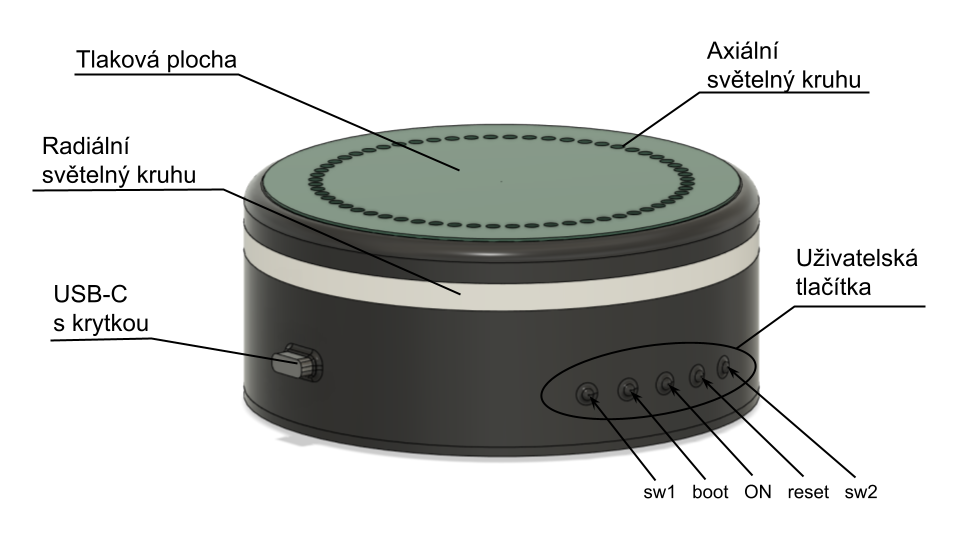
\includegraphics[width=\textwidth]{text/PraktickaCast/img/AHS-nacrt.png}
    \caption{Návrh vzhledu zařízení}
    \label{fig:AHS-nacrt}
\end{figure}

\newpage
\section{Struktura elektroniky základní jednotky}

Elektronika je rozdělena na dvě samostatné PCB.
Jde o~hlavní desku, na které je většina elektroniky a o~desku s~hlavním uživatelským rozhraním (LED deska).

Původně jsem uvažoval ještě třetí desku, se základním uživatelským rozhraním (mini~UI) pro usnadnění zajištění jisté míry voděodolnosti, ale nakonec jsem se rozhodl spojit ji s hlavní deskou.

\subsection{LED deska}
Na LED desce se nacházejí oba světelné kruhy a~elektronika pro snímání tlakové plochy, tedy LDC1614 \cite{LDC1614} a~jeho snímací LC články.
Právě snímaní tlakové plochy je jeden z~hlavních důvodů oddělení této elektroniky na samostatnou desku, zabere totiž docela dost prostoru.

\begin{itemize}
    \item Axiální LED kruh z~60 RGB LED WS2812
    \item Radiální LED kruh z~60 RGB LED WS2812
    \item LDC1614 nebo LDC1314 se čtyřmi snímacími LC články pro snímání tlakové plochy
    \item konektor na propojení s~hlavní deskou
\end{itemize}

\subsection{Hlavní deska}
Na hlavní desce je většina systému základního zařízení.

Řídící mikrokontroler AHS je ESP32-S3 (výběr viz \ref{subs:vyberMikrokontroleru}).

Zdroj AHS je tvořen dvěma LiIon články 18650 v~paralelním uspořádání.
Paralelní uspořádání jsem zvolil tak, aby nebylo nutné řešit balancování článků.

Aby nebylo možné softwarově baterii podvybít, má AHS ochranu podvybitím, která celé zařízení vypne v~případě, že dojde k~vybití baterie pod 2.8V.
Pochopitelně software by měl vybitou baterii zaznamenat mnohem dřív a~chovat se podle toho, např. neumožnit spustit hru s~baterií při napětí 3.0V.

Na hlavní desce je i~nabíjecí elektronika.
Navíc, aby se minimalizoval čas nabíjení, zařízení podporuje standard Power Delivery a~to až do napětí 14V.

Protože různé periferie vyžadují různá napájecí a~komunikační napětí, je na hlavní desce hned pět napájecích větví.
\begin{itemize}
    \item VCC, napětí baterie sloužící jako zdroj pro ostatní napájecí větve a~pro napájení komunikačního modulu. 
    \item Napětí \(3.3\-[V]\) na napájení logické části celého základního zařízení.
    \item Napětí \(5.0\-[V]\) pro LED desku a~externí moduly
    \item Napětí \(1.8\-[V]\) pro napájení napěťových převodníků sloužících na komunikaci s~komunikačním modulem 
    \item V-USB, napětí \(5\- - \-21\-[V]\) z~USB-C konektoru pro nabíjení a~programování
\end{itemize}
Napětí větví \(3.3\-[V]\) a~\(1.8\-[V]\) je tvořeno pomocí LDO.
Na vytvoření větve \(5\-[V]\) je ale potřeba spínaný zdroj a~to primárně ze dvou důvodů.
Za prvé protože napětí baterie, ze které se tato větev napájí, má nižší napětí a~je jej tedy třeba vyspínat na napětí vyšší.
Za druhé tento zdroj poskytuje do systému mnohem větší proudy než druhé dvě větve a~bylo by tedy vhodné použít spínaný zdroj i~v případě vyžšího vstupního napětí.

\newpage
Na hlavní desce je také řada konektorů sloužící pro připojení ostatních systémů.
Jde o~konektory na:
\begin{itemize}
    \item propojení s~LED deskou                                            % samostatný objekt
    \item komunikační modul (M2 Konektor umožňuje použít různé moduly)      % externě definovaný objekt
    \item externí moduly                                                    % samostatný objekt
    \item USB-C (nabíjení a~programování AHS)                               % externě definovaný objekt
    \item programátor                                                       % samostatný objekt
\end{itemize}
Do konektorů by se dal zařadit i~držák na dva LiIon články 18650.

Jako jednoduchý zvukový výstup je na desce také piezoměnič.

\subsection{Výběr mikrokontroleru \label{subs:vyberMikrokontroleru}}
Požadavky na mikrokontroler jsou:
\begin{itemize}
    \item WiFi
    \item Bluetooth
    \item alespoň 3~UARTy
    \item alespoň 30 GPIO pinů
    \item I2C
    \item dostatečný výpočetní výkon pro hladký chod interpretru JavaScriptu nebo Pythonu
\end{itemize}

Dostupných možností je nespočet ale pro příklad mohu uvést:
\begin{figure}[h]
    \hspace{-20mm}
    \small
    \begin{tabular}{|l|l|l|l|l|c|}
        \hline
        Mikrokontroler                   & Jádro         & Počet GPIO pinů    & Počet UARTů   & Počet I2C & Wi-Fi a Bluetooth                \\ \hline
        ESP32        \cite{ESP32}        & 2x Xtensa LX6 & 34                 & 3             & 2         & \textcolor{green}{\checkmark}    \\ \hline
        ESP32-S3     \cite{ESP32S3}      & 2x Xtensa LX7 & 45                 & 3             & 2         & \textcolor{green}{\checkmark}    \\ \hline
        ESP32-C6     \cite{ESP32C6}      & 1x RISC-V     & 34                 & 3             & 2         & \textcolor{green}{\checkmark}    \\ \hline
        PIC32MZ-W1   \cite{PIC32MZ}      & DS60001192    & 62                 & 3             & 2         & \textcolor{green}{\checkmark}    \\ \hline

        \textcolor{red}{nRF7000      \cite{nRF7000}}      & -             & \textcolor{red}{13}& \textcolor{red}{0} & \textcolor{red}{0}    & \textcolor{green}{\checkmark}    \\ \hline
        \textcolor{red}{RTL8710      \cite{RTL8710}}      & ARM Cortex-M3 & \textcolor{red}{17}& \textcolor{red}{1} & 3                     & \textcolor{green}{\checkmark}    \\ \hline
        \textcolor{red}{RTL8721DM    \cite{RTL8721DM}}    & -             & \textcolor{red}{17}& 3                  & 2                     & \textcolor{green}{\checkmark}    \\ \hline
        \textcolor{red}{STM32WB55    \cite{STM32WB55}}    & ARM Cortex-M4 & 37                 & \textcolor{red}{1} & 2                     & \textcolor{red}{$\times$}        \\ \hline
        \textcolor{red}{MSP430BT5190 \cite{MSP430BT5190}} & -             & 32                 & 4                  & 4                     & \textcolor{red}{$\times$}        \\ \hline
    \end{tabular}
    \caption{Dostupné vyhovující mikrokontrolery}
    \label{tab:vyberMikrokontroleru}
\end{figure}

Abych nemusel řešit anténu použil bych mikrokontroler na modulu, který má anténu integrovanou, a navíc řeší i flash paměť. 
Protože už tyto moduly interně používají některé GPIO, klesne množství, které mohu využít.

\begin{figure}[h]
    \centering
    \begin{tabular}{|l|l|l|l|l|}
        \hline
        Mikrokontroler                  & Počet GPIO pinů    & vyhovuje?                     \\ \hline
        ESP32-WROOM     \cite{ESP32}    & 26                 & \textcolor{red}{$\times$}     \\ \hline
        ESP32-S3-WROOM  \cite{ESP32S3}  & 36                 & \textcolor{green}{\checkmark} \\ \hline
        ESP32-C6-WROOM  \cite{ESP32C6}  & 23                 & \textcolor{red}{$\times$}     \\ \hline
        WFI32E01PC      \cite{PIC32MZ}  & 37                 & \textcolor{green}{\checkmark} \\ \hline
    \end{tabular}
    \caption{Moduly s mikrokontrolery}
    \label{tab:ModulySMikrokontrolery}
\end{figure}

Jedním z požadavků na zařízení je dostatečný výpočetní výkon pro hladký chod interpretru JavaScriptu nebo Pythonu.
Výpočetní výkon se porovnává poněkud složitěji, protože se nejedná tak úplně o~jeden parametr.
V tomto případě je ale vhodné prozkoumat i dostupnost interpretru pro daný mikrokontroler.
Pro ESP32-S3 je dostupný JavaScriptový interpreter Jaculus \cite{Jaculus} i~interpretr jazyka Python MicroPython \cite{MicroPythonESP32S3}.
Pro PIC32MZ-W1 je dostupný interpreter jazyka Python MicroPython \cite{MicroPythonPIC32MZ-W1}, interpretter JavaScriptu jsem však nenašel.
ESP32-S3 mi tak poskytuje výhodu v možnosti volby skriptovacího jazyka.

Další výhodou ESP32-S3 je jeho cena, která se pohybuje okolo \(4\-\$\) \cite{JSC-ESP32-S3}.
PIC32MZ-W1 je u JLCPCB za \(13.65\-\$\) \cite{JSC-WFI32}.
Navíc u JLCPCB je PIC32MZ-W1 sice v nabídce, ale není na skladě \cite{JSC-WFI32}, zatímco u ESP32-S3 je aktuálně dostupných hned 19 variant \cite{JSC-ESP32-S3}.

V mém případě má ESP32-S3 ještě jednu podstatnou výhodu, a tou je fakt, že s rodinou mikrokontrolerů ESP32 mám dlouholeté zkušenosti.
Z těchto důvodu jsem se rozhodl pro ESP32-S3.

\subsection{Propojení hlavní desky a~LED desky}
Mezi hlavní deskou a~LED deskou je třeba převést napájení a~několik signálů.
LED deska vyžaduje na konektoru přítomnost dvou napájecích větví \(5\-[V]\) pro světelné kruhy a~\(3.3\-[v]\) pro snímání tlakové plochy.
Protože do LEDek může téct proud až 5A a~může být zároveň i~docela rychle spínaný, považuji za rozumné oddělit napájecím větvím zem.
Oddělení je tedy provedeno už na konektoru hlavní desky aby se omezilo rušení na napájení snímání tlakové plochy.

Na samotné propojení jsem se rozhodl použít FFC kabel s~roztečí \(0.5\-[mm]\), pro jeho rozměry a cenovou dostupnost.
Jedním vodičem takovéhoto kabelu lze vést proud maximálně \(0.4\-[A]\) \cite{FFC-konektor}.
Protože ale potřebuji dodat proud až 5A, použiji 13 vodičů vedle sebe jakožto nejmenší počet, který přenese požadovaný proud v~rámci daných mezí.

Mimo napájení je tímto propojením veden i~signál s~daty pro světelné kruhy a~I2C sběrnice s~interruptem pro připojení čipu LDC1614 \cite{LDC1614}.

Vzhledem k~počtu potřebných vodičů (konkrétně 32) jsem se rozhodl použít běžný FFC konektor se 40 kontakty s~tím, že zbylé kontakty se mohou hodit v~budoucnu.

\subsection{Modulový konektor \label{sec:ModulovyKonektor}}
Modulovým konektorem je vedeno \(5\-[V]\) jako napájení pro moduly a~UART s~interruptem pro komunikaci.

Nad volbou komunikační sběrnice jsem strávil poměrně dost času přemýšlením.
Původně jsem uvažoval o~využití RS485 jakožto odolné sběrnice, u~které by v~případě potřeby nemusel být problém ani delší kabel.
RS485 má ale nevýhodu v~tom, že potřebuje dodatečný hardware, kterému bych se hlavně na modulech rád vyhnul.
Stejný problém nastal u~CANu a~USB, které by navíc mělo výhodu kompatibility s~velkým množstvím hotových zařízení.

V~první úvaze o~UARTu jsem jej nejprve zavrhl kvůli potenciální náročnosti na přeposílání dat mezi moduly.
Při standardním použití bych totiž moduly řadil za sebe.
Prvnímu modulu by tak chodili data pro všechny ostatní moduly a~musel by je přeposílat dál, což by mohlo stát nezanedbatelné množství procesorového času.
V~jisté chvíli jsem ale narazil na nestandardní komunikaci pomocí UARTu implementované v~projektu Servio \cite{Servio}.
Tato implementace používá UART jako sběrnici.
Namísto standardního použití pro komunikace jeden s~jedním tak může komunikovat jeden s~více.
Na tomto řešení je výhodné, že nevyžaduje žádný dodatečný hardware a~prakticky každý dnešní mikrokontroler je možné k~této sběrnici velmi snadno připojit.
Ve srovnání s~RS485 je sice mnohem méně odolná proti rušení, ale uvnitř zařízení nebude linka vedena na víc než malé desítky centimetrů.
Komunikace na delším kabelu je pak jednoduše nahraditelná bezdrátovou komunikací a~není tak potřebné, aby to musela tato sběrnice ze základu podporovat.
Každopádně v~případě potřeby delšího kabelu je možné navrhnout externí modul, který s~této sběrnice velmi jednoduše udělá RS485 pro externí využití.
Alternativně by se pro komunikaci na delším kabelu dalo použít USB, které je společně s~nabíjením přivedeno na USB-C.

Všechny moduly jsou tedy připojeny na jeden RX pin AHS.
Proto musí firmware AHS zajistit, aby dva moduly nevysílaly současně.
Aby se zabránilo možným zkratům, jako ochranu má každý modul své piny UARTu připojeny přes rezistor \(180\-[\Omega]\).
Interrupt pin modulů se naopak chová jako open-collector a~na straně hlavního zařízení je na něj tedy připojen pull-up rezistor.
Abych alespoň trochu zvýšil odolnost linky proti rušení, přidám na přijímací stranu pull-up rezistor.
Cílem je zvýšení komunikačního proudu, aby se případný proud vyvolaný rušením neprojevil.
V~neposlední řadě mají všechny piny na konektoru ESD ochranu.

\newpage
\subsection{Konektor programátor}
Zařízení se dá jednoduše programovat přes USB-C, tento kanál se ale dá softwarově narušit a~pro takové případy je tu konektor na programátor.
Jde o~šest plošek, na které se programátor připojuje pomocí pružinkovích kontaktů.
Programátor sice obsahuje jen jednoduchou elektroniku, která by mohla být i~přímo v~elektronice AHS, ale ve většině případů by byla zbytečná.
Ve chvíli, kdy by byla potřeba, je stejně nutná odborná obsluha a~pro tu není problém použít programátor.

\subsection{USB-C}
Jako napájecí a~programovací konektor je použito USB-C.
Díky němu je možné podporovat standard Power Delivery využitý pro zrychlení nabíjení.
Konektor je ale použit i~na pohodlnější programování zařízení, bez potřeby programátoru.

\subsection{Konektor komunikačního modulu}
Pro připojení komunikačního modulu jsem zvolil konektor M2 typ-B jakožto standard pro tyto moduly.
Díky tomuto konektoru mohu jednoduše připojit různé LTE a~GNSS moduly.

\subsection{Mechanické uspořádání}

